\documentclass{article}

\usepackage{amsmath}
\usepackage{graphicx}
\usepackage{xcolor}
\usepackage[export]{adjustbox}
\RequirePackage[margin=1in]{geometry}

\newcommand\todo[1]{\textcolor{red}{TODO: #1}}

\newcommand\animation[1]{\textcolor{blue}{ANIMATION: #1}}

\begin{document}
	
\title{Hillshade Video Script}
\author{Nathan Stouffer}
\date{}
\maketitle

\section{Intro}

\subsection{Motivation}

Despite the simplicity of the map below, I'm betting that you are able to discern a lot of information about this region.
You can probably see that this spot is relatively flat and this other area is pretty steep.
Maybe you can pick out a gully right here and a ridgeline over here.
Or possibly you've noticed that this face is pretty rugged while this slope is not quite as technical
Regardless of what features you've noticed, I'm certain you have some notion of what this terrain looks like even though all you are looking at is a greyscale image.
In fact, I'd be willing to bet that your understanding of this map is better than if I had given you contour lines even though that is a more precise way to convey information.

\animation{Bring in more maps (one with just contours and another with contours/hillshade)}

This map is intentionally set up so that your brain can intuit the shape of the terrain.
Modern computers do much of this work today, but cartographers have been using versions of this technique for hundreds of years.
And many other applications use similar strategies to help convey geometric information.

The topic I'd like to discuss today is a lighting technique called hillshade.
We're going to talk about why it's such an effective method of illuminating terrain and walk through the math that powers it.

\begin{center}
	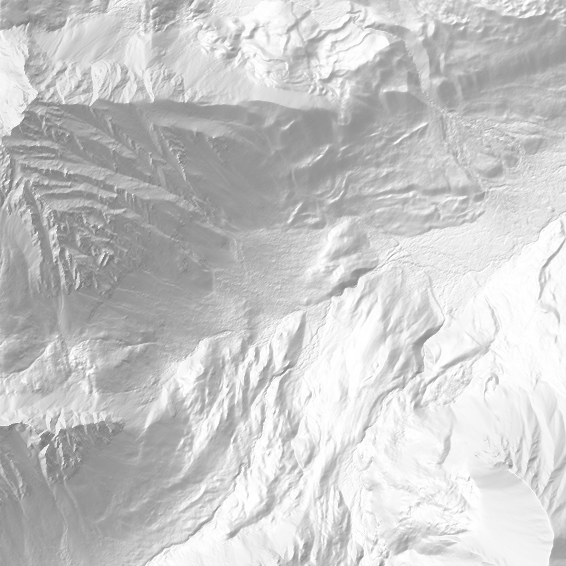
\includegraphics[width=0.5\textwidth,frame]{assets/hillshade-example.png}
\end{center}

\subsection{Directional Lighting}

The particular topic we'll be discussing is hillshade, but it's worth mentioning that hillshade is a very specific example of something called a directional light.
Directional lights are used all over computer graphics and are themselves just one option for how you might want to light a scene.
What I find so intriguing about directional lights is that they give you a lot of bang for your buck.
They give you quite a bit of realism for the amount of effort that you need to expend.

\animation{Fade in a graph similar to the below image.}

\begin{center}
	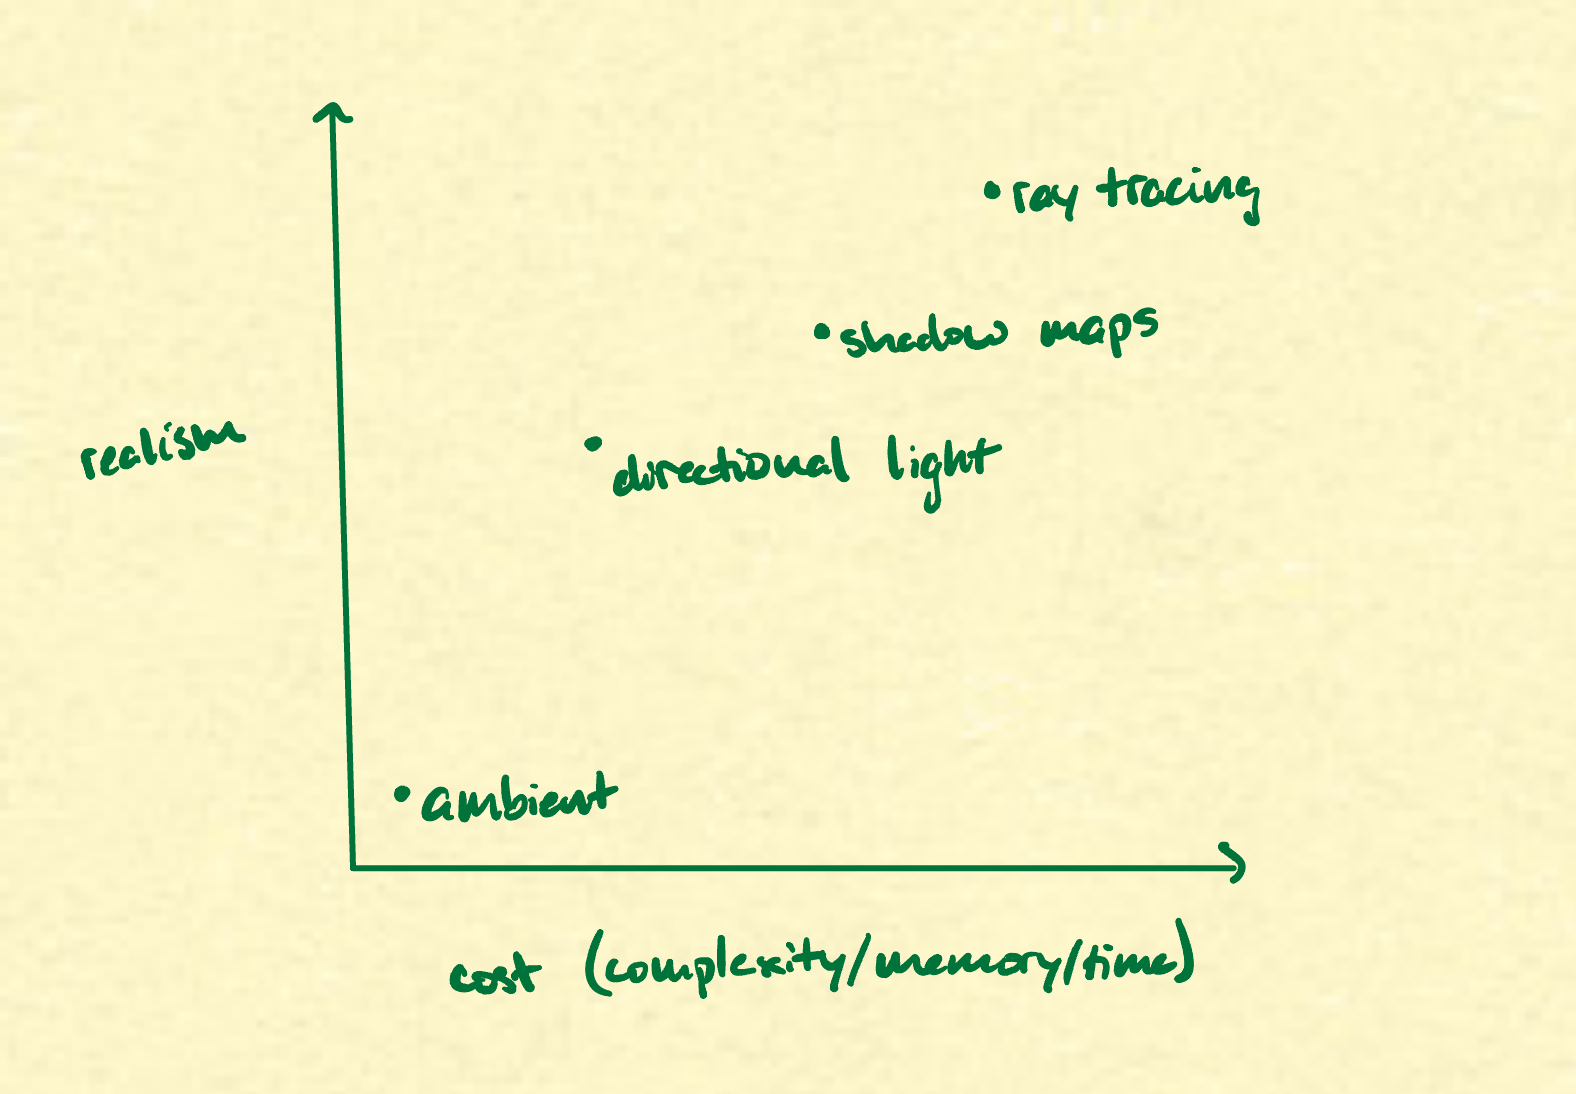
\includegraphics[width=0.65\textwidth,frame]{assets/realism.jpg}
\end{center}

If you were to represent different lighting techniques as points in the plane where the y-axis represents some notion of realism and the x-axis represents some notion of cost (maybe in terms of complexity/memory/computation time).
Then on that graph, directional lights would exist at a sweet spot where they are unreasonably effective -- they don't cost that much but they provide a healthy amount of realism.

So what is a directional light?
It is a pseudo-realistic model of how light behaves.
In the interest of simplicity, directional lights take a few shortcuts via some assumptions:

\begin{enumerate}
	
\item First, we ignore obstructions.
What this means is that we aren't computing true shadows -- just whether or not terrain \textit{faces} the light.
The direction is all that matters.
\animation{Demonstrate a simple example of shadows in 2D}.
	
\item The second assumption is that we assume the light source to be extremely far away.
If that is the case, every point in the scene has light coming from the same direction -- giving the technique its name.
You can imagine a directional light as an effect where we light up areas that face the light and shadow areas that don't.
The light direction is given to us by configuration.
To make the math a little simpler, I am going to use the negative of the light direction.
This is the vector $l$ that points directly \textit{towards} the light source.

\end{enumerate}

The direction that the terrain faces is encoded in something called a surface normal.
The surface normal at any particular point is the vector that orthogonal to the plane that approximates a very small region around that point.

\animation{Show a rotating plane with a surface normal that is lit according to hillshade.}

When zoomed in on a small region of the terrain with surface normal $n$, the effect we are looking for should behave like this:
If $n$ generally points in the same direction as $l$, we want a strong amount of light.
If $l$ kind of glances off the terrain, we want half-strength light.
And if $n$ generally points in the opposite of $l$, we want very little light.

\section{Hillshading}

At this point, we've covered what the effect should do, but how can we accomplish it?
what are the nuts and bolts that turn this loose discussion into a sequence of mathematical operations?

\subsection{Cosine}

We can start by being more precise about describing how the light strength should vary.
Let's represent a small area of the terrain as a rotated square.
When $n$ and $l$ point in the exact same direction, we want to light at full strength.
And we know we want to decrease the strength of the light as the angle between $n$ and $l$ increases.
To root some of our model in reality, it would be a good idea to decrease the strength of the shadow based on how much light is blocked by the rotated square.
The amount of light that is blocked is the area of the shadow.

I won't prove this for you, but it so happens that the signed area of the rotated square's shadow is $\cos \theta * A$ where $A$ is the area of the original plane and the sign encodes whether or not the plane faces the light source.
If an un-rotated plane gets the full light strength $1$, then a rotated plane gets strength $1 * \cos \theta = \cos \theta$.

You might notice that $\cos \theta$ can be negative.
What are we to do with a negative light strength?
Some directional light models ignore negative light strengths.
Hillshade takes a slightly different approach.
Our goal is to effectively light a map so that the reader can see terrain features.
When we ignore negative light strength, we effectively remove shading on all terrain that faces away from the light source.
Instead, it is more effective to remap the range of cosine to the interval $[0, 1]$.
This can be done by $\dfrac{1}{2}(1 + \cos \theta)$.
 
\animation{Transform the range of cosine}

\begin{center}
	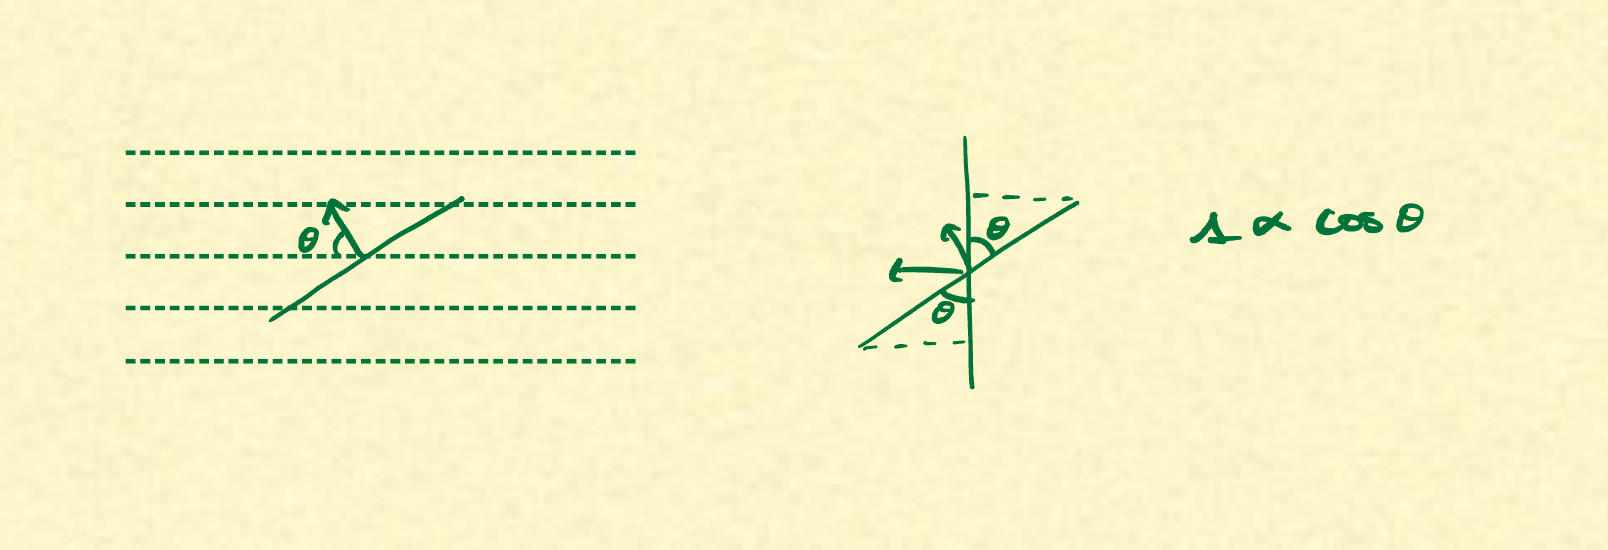
\includegraphics[width=0.75\textwidth,frame]{assets/cosine.jpg}
\end{center}

\subsection{Law of Cosines $=>$ Dot Product}

We now know that we want to vary the strength of our lighting according to $\cos \theta$.
But that doesn't really help us much because we don't know what $\theta$ is -- all we know are the vectors $l$ and $n$.
At the end of the day, those are just lists of numbers.
What is the link between these two vectors and cosine?

If we were solving this on our own, we would need to start experimenting and see if inspiration strikes.
It might take a lot of tries and result in quite a few dead ends.
It's one of those things where experience is the best teacher.

... But if I were to offer one piece of advice, I would say it's often worth constructing a triangle.
Maybe it's the types of problems that I interact with, but I find triangles to be an extremely effective tool.
In this case, we are going to draw the third leg of our triangle here and use the Law of Cosines.

\begin{center}
	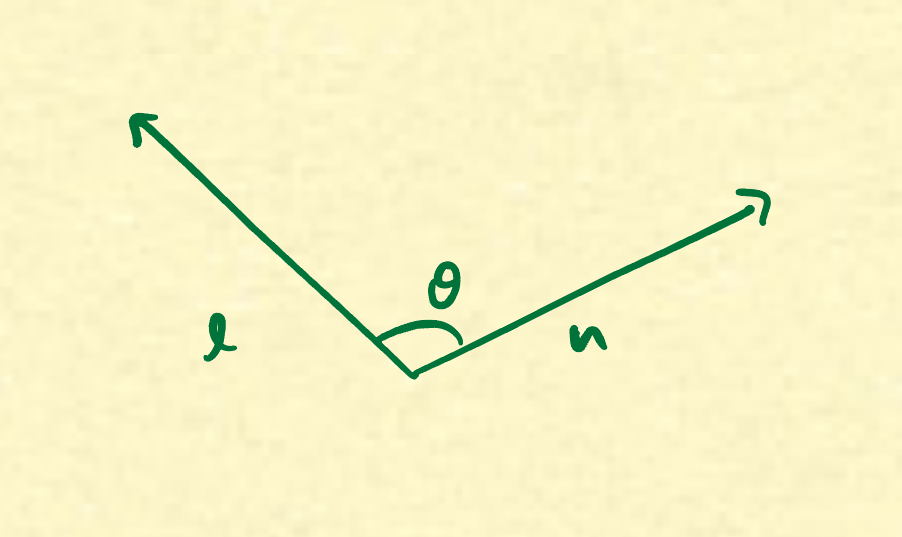
\includegraphics[width=0.3\textwidth,frame]{assets/ln.jpg}
	\hspace{0.2\textwidth}
	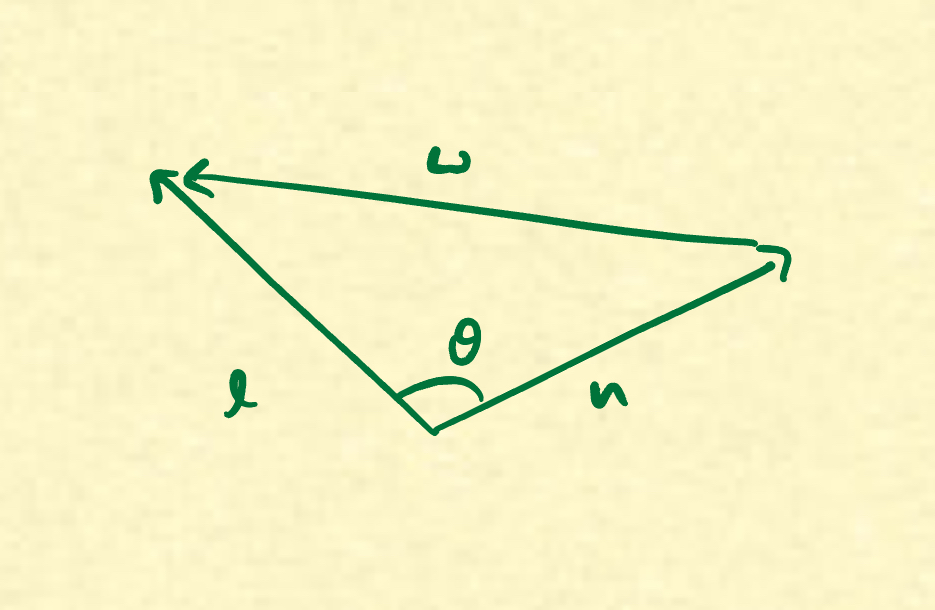
\includegraphics[width=0.2735\textwidth,frame]{assets/lnw.jpg}
\end{center}

The full Law of Cosines says that for any triangle with angles/sides labeled like so, we have $c^2 = a^2 + b^2 - 2ab \cos C$.
In our case, $a = |l|$, $b = |n|$, and $C = \theta$.
The third side is the difference between $l$ and $n$ so its length is $| l - n |$.

\begin{align*}
|l-n|^2 = |l|^2 + |n|^2 - 2 |l| |n| \cos \theta & \quad \text{substitute from generalized LoC} \\
|l-n|^2 = 2 - 2 \cos \theta & \quad \text{since we know } |l| = |n| = 1 \\
1 - \dfrac{1}{2}|l-n|^2 = \cos \theta & \quad \text{simplifying}
\end{align*}

Using the Law of Cosines, we are now able to compute $\cos \theta$ just from the values of $l$ and $n$.
Those of you who are familiar with the dot product know that this can be simplified further (resulting in some extremely efficient code).
But in the interest of accessibility, I am going to leave it here.

\section{Final product}

So now we have the final product!
From earlier, we know that we want to light the terrain according to $\dfrac{1}{2}(1 + \cos \theta)$ and we just proved that we can compute $\cos \theta$ as $1 - \dfrac{1}{2}|l-n|^2$.
That's all it takes to produce the beautiful hillshade effect shown in these images.
It never ceases to amaze me how such simple computation can produce such stunning and realistic images.

\animation{Show a few examples.}

\section{Endnotes}

I'd like to close the video by making a few comments.

\subsection{Modified techniques}

Hillshading isn't just one thing.
It is actually a term for a family of effects that can be applied to a map.
There are a lot of variations out there.
Some examples include ambient lighting, exaggerating the normal vector, using multiple light sources, and playing around with colored lights.
You now have the mathematical framework that sits behind all of them.

\todo{Possibly mention Eduard Imhof.}

\subsection{Pseudoscopic Illusion}

Most people recognize features better when directional lights are placed in the top left of an image.
Because many maps use a north-up convention, hillshade is typically lit from the northwest.

However, this can some backfire when a map with static hillshade is oriented with a south-up convention.
When that occurs, your brain might interpret everything backwards (id valleys as ridges and ridges and valleys).
This is called a pseudoscopic illusion.

\animation{Show a south-up map light from the northwest and then fade in the same map (still south up) with a southeast (top left) light}.

\subsection{Simplicity}

My final comment has to do with the simplicity of this effect.
All the maps you've been viewing are 2-dimensional -- and I don't just mean that the screen you're viewing is 2-dimensional.
I mean that the actual model that I am rendering is 2D.

\animation{Pitch the camera}

Despite that, it is an incredibly effective method of conveying information about terrain.
I find that fascinating.

\animation{3D flythrough?}

\end{document}